\documentclass[11pt]{article}

% ----------------------------------------------------------
% PACKAGES
% ----------------------------------------------------------
\usepackage[T1]{fontenc}
\usepackage[utf8]{inputenc}
\usepackage{lmodern}
\usepackage[margin=1in]{geometry}
\usepackage{amsmath, amssymb}

\usepackage{adjustbox}
\usepackage{graphicx}
\usepackage{xcolor}
\usepackage{booktabs}
\usepackage{enumitem}

% --- Tables that auto-fit \textwidth ---
\usepackage{tabularx}

% TikZ + PGFPLOTS (REQUIRED FOR FIGURES)
\usepackage{tikz}
\usepackage{pgfplots}
\pgfplotsset{compat=1.18}
\usepgfplotslibrary{groupplots}

\usepackage{framed}
\usepackage{setspace}
\usepackage{microtype}
\usepackage[hidelinks]{hyperref}
\usepackage[authoryear]{natbib}

% ----------------------------------------------------------
% CUSTOM MACROS (shared notation)
% ----------------------------------------------------------
% ==========================================================
% EB-PAPERS: CANONICAL MACROS / COMMANDS
% Forecast Readiness Framework (FRF) / Electric Barometer
% ==========================================================
% Goals:
% - One meaning per symbol.
% - Shared across all papers/notes/briefs.
% - Backwards-compatible aliases.
% - Avoid redefinition errors via \providecommand.
% ==========================================================

% ----------------------------------------------------------
% Core framework / artifacts
% ----------------------------------------------------------
\providecommand{\FRF}{\ensuremath{\mathrm{FRF}}}
\providecommand{\FRS}{\ensuremath{\mathrm{FRS}}}

\providecommand{\FPC}{\ensuremath{\mathrm{FPC}}}
\providecommand{\DQC}{\ensuremath{\mathrm{DQC}}}
\providecommand{\Governance}{\ensuremath{\mathrm{Governance}}}
\providecommand{\GovernanceDecision}{\ensuremath{\mathrm{GovernanceDecision}}}

\providecommand{\RAL}{\ensuremath{\mathrm{RAL}}}

% Readiness primitives / governance vocabulary
\providecommand{\ReadinessPrimitive}{\ensuremath{\mathrm{RP}}}

% Limited-Time Offers
\providecommand{\LTO}{\ensuremath{\mathrm{LTO}}}
\providecommand{\LTOs}{\ensuremath{\mathrm{LTOs}}}

% ----------------------------------------------------------
% Core metrics (upright math)
% ----------------------------------------------------------
\providecommand{\CWSL}{\ensuremath{\mathrm{CWSL}}}
\providecommand{\CWSLR}{\ensuremath{\mathrm{CWSLR}}} % named artifact in prose
\providecommand{\NSL}{\ensuremath{\mathrm{NSL}}}
\providecommand{\UD}{\ensuremath{\mathrm{UD}}}
\providecommand{\HR}{\ensuremath{\mathrm{HR}}}
\providecommand{\HRtau}{\ensuremath{\mathrm{HR}@\tau}}

% FRS sub-terms
\providecommand{\CWSLscaled}{\ensuremath{\mathrm{CWSL}_{\mathrm{scaled}}}}
\providecommand{\CWSLmax}{\ensuremath{\mathrm{CWSL}_{\max}}}

% Legacy HR macro names
\providecommand{\HRAT}{\ensuremath{\mathrm{HR@\tau}}}
\providecommand{\tauTol}{\ensuremath{\tau}}
\providecommand{\tauop}{\ensuremath{\tau}}

% ----------------------------------------------------------
% Indexing and sets
% ----------------------------------------------------------
\providecommand{\Iset}{\ensuremath{I}}
\providecommand{\Tset}{\ensuremath{T}}

\providecommand{\entity}{\ensuremath{i}}
\providecommand{\timeindex}{\ensuremath{t}}

% Back-compat index shorthands
\providecommand{\iidx}{\entity}
\providecommand{\tidx}{\timeindex}

% Summation shorthand
\providecommand{\sumit}{\ensuremath{\sum_{\entity \in \Iset} \sum_{\timeindex \in \Tset}}}

% Optional sizes / counts
\providecommand{\Tsize}{\ensuremath{|\Tset|}}
\providecommand{\nobs}{\ensuremath{N}}

% ----------------------------------------------------------
% Forecast / demand notation
% ----------------------------------------------------------
\providecommand{\y}{\ensuremath{y}}
\providecommand{\yhat}{\ensuremath{\hat{y}}}

\providecommand{\yit}{\ensuremath{y_{\entity\timeindex}}}
\providecommand{\yhatit}{\ensuremath{\hat{y}_{\entity\timeindex}}}

% Common residuals / errors
\providecommand{\errit}{\ensuremath{e_{\entity\timeindex}}}
\providecommand{\resit}{\errit} % alias
\providecommand{\absit}{\ensuremath{\left|\yhatit - \yit\right|}}
\providecommand{\abserrit}{\absit} % alias

% Explicit residual definition macro (optional)
\providecommand{\resdef}{\ensuremath{\errit = \yit - \yhatit}}

% ----------------------------------------------------------
% Shortfall / overbuild decomposition
% ----------------------------------------------------------
\providecommand{\shortfall}{\ensuremath{s}}
\providecommand{\overbuild}{\ensuremath{o}}

\providecommand{\sit}{\ensuremath{s_{\entity\timeindex}}}
\providecommand{\oit}{\ensuremath{o_{\entity\timeindex}}}

% Positive-part operator (canonical name)
\providecommand{\pospart}[1]{\left(#1\right)_{+}}

% Explicit decompositions
\providecommand{\shortfalldef}{\ensuremath{\sit = \pospart{\yit - \yhatit}}}
\providecommand{\overbuilddef}{\ensuremath{\oit = \pospart{\yhatit - \yit}}}

% Back-compat convenience symbols used in some notes
\providecommand{\sdepth}{\shortfall} % UD paper convenience

% ----------------------------------------------------------
% Indicators / expectations / operators
% ----------------------------------------------------------
% Canonical indicator: \Ind{event}
\providecommand{\Ind}{\ensuremath{\mathbb{I}}}
\providecommand{\indicator}[1]{\ensuremath{\mathbf{1}\{#1\}}} % prose-friendly alternative

% Back-compat: some notes used \Indicator (capital I). Keep as an alias to the
% canonical \Ind to avoid duplicate meanings.
\providecommand{\Indicator}{\Ind}

% If you want function-style indicator without braces: \Ind\!(event)
% Keep as \Ind and let authors decide.
\providecommand{\E}{\ensuremath{\mathbb{E}}}

\providecommand{\abs}[1]{\left|#1\right|}
\providecommand{\card}[1]{\left|#1\right|}

% ----------------------------------------------------------
% Cost parameters + cost ratio calibration (CWSLR note)
% ----------------------------------------------------------
% IMPORTANT: Canonical costs are subscripted (c_u, c_o). This avoids
% collisions with superscript variants.
\providecommand{\cu}{\ensuremath{c_u}}
\providecommand{\co}{\ensuremath{c_o}}

% Entity-specific costs
\providecommand{\cui}{\ensuremath{c_{u,\entity}}}
\providecommand{\coi}{\ensuremath{c_{o,\entity}}}

% Cost ratio
\providecommand{\R}{\ensuremath{R}}
\providecommand{\Ri}{\ensuremath{R_{\entity}}}
\providecommand{\Rdef}{\ensuremath{R = \cu/\co}}

% Aggregate under/over cost functions (used in calibration prose)
\providecommand{\UnderCost}{\ensuremath{\mathrm{UnderCost}}}
\providecommand{\OverCost}{\ensuremath{\mathrm{OverCost}}}

% Candidate grid
\providecommand{\Rgrid}{\ensuremath{\mathcal{R}}}

% Calibrated selections
\providecommand{\Rstar}{\ensuremath{R^{\ast}}}
\providecommand{\Rist}{\ensuremath{R^{\ast}_{\entity}}}

% CWSL as a function of R (notation)
\providecommand{\CWSLofR}{\ensuremath{\CWSL(\R)}}
\providecommand{\CWSLofRi}{\ensuremath{\CWSL(\Ri)}}

% Balance-based selection operator (kept as a macro because you used it)
\providecommand{\Rbalance}{%
\ensuremath{%
\arg\min_{\R \in \Rgrid}\left|\UnderCost(\R) - \OverCost(\R)\right|%
}%
}

% Back-compat (older notes used superscripts c^u / c^o)
\providecommand{\cuSup}{\ensuremath{c^{u}}}
\providecommand{\coSup}{\ensuremath{c^{o}}}
\providecommand{\cuiSup}{\ensuremath{c^{u}_{\entity}}}
\providecommand{\coiSup}{\ensuremath{c^{o}_{\entity}}}

% ----------------------------------------------------------
% HR@tau scanning / calibration (HRtau note)
% ----------------------------------------------------------
\providecommand{\tauval}{\ensuremath{\tau}}
\providecommand{\tauv}{\tauval}
\providecommand{\taui}{\ensuremath{\tau_{\entity}}}

% Candidate tolerance grid
\providecommand{\TauGrid}{\ensuremath{\mathcal{T}}}

% Calibrated tolerances
\providecommand{\taustar}{\ensuremath{\tau^{\ast}}}
\providecommand{\taustari}{\ensuremath{\tau^{\ast}_{\entity}}}

% Target hit-rate (if used)
\providecommand{\hstar}{\ensuremath{h^{\ast}}}

% Hit indicator definition helpers
\providecommand{\Hitit}{\ensuremath{h_{\entity\timeindex}}}
\providecommand{\HitDef}{\ensuremath{\Hitit = \Ind\!\left(\absit \le \tauval\right)}}

% HR as a function of tau
\providecommand{\HRoftau}{\ensuremath{\HR(\tauval)}}
\providecommand{\HRtauoftau}{\ensuremath{\HRtau(\tauval)}}

% Optional utility selection helpers
\providecommand{\lambdau}{\ensuremath{\lambda}}
\providecommand{\taumax}{\ensuremath{\tau_{\max}}}
\providecommand{\Utility}{\ensuremath{\mathcal{U}}}
\providecommand{\UtilityDef}{\ensuremath{\Utility(\tauval) = \HR(\tauval) - \lambdau \cdot (\tauval/\taumax)}}

% Governance guards
\providecommand{\taufloor}{\ensuremath{\tau_{\min}}}
\providecommand{\taucap}{\ensuremath{\tau_{\mathrm{cap}}}}
\providecommand{\nmin}{\ensuremath{n_{\min}}}

% ----------------------------------------------------------
% DQC / snapping / quantization (DQC note)
% ----------------------------------------------------------
\providecommand{\gunit}{\ensuremath{g}}
\providecommand{\guniti}{\ensuremath{g_{\entity}}}

\providecommand{\ygrid}{\ensuremath{\tilde{y}}}
\providecommand{\ygridit}{\ensuremath{\tilde{y}_{\entity\timeindex}}}

\providecommand{\yhatgrid}{\ensuremath{\tilde{\hat{y}}}}
\providecommand{\yhatgridit}{\ensuremath{\tilde{\hat{y}}_{\entity\timeindex}}}

\providecommand{\snap}{\ensuremath{\mathcal{S}}}
\providecommand{\snaphatdef}{\ensuremath{\yhatgridit = \snap_{\gunit}\!\left(\yhatit\right)}}
\providecommand{\snapydef}{\ensuremath{\ygridit = \snap_{\gunit}\!\left(\yit\right)}}

\providecommand{\residit}{\ensuremath{r_{\entity\timeindex}}}
\providecommand{\residdef}{\ensuremath{\residit = \yit - \ygridit}}

\providecommand{\MAD}{\ensuremath{\mathrm{MAD}}}
\providecommand{\IQR}{\ensuremath{\mathrm{IQR}}}

\providecommand{\multirate}{\ensuremath{\rho}}
\providecommand{\multiratei}{\ensuremath{\rho_{\entity}}}

\providecommand{\DeltaStar}{\ensuremath{\Delta^{\ast}}}

\providecommand{\Pset}{\ensuremath{\mathcal{P}}}
\providecommand{\packunit}{\ensuremath{p}}
\providecommand{\packuniti}{\ensuremath{p_{\entity}}}

% DQC classes
\providecommand{\ContinuousLike}{\textsc{Continuous-like}}
\providecommand{\Quantized}{\textsc{Quantized}}
\providecommand{\PiecewisePacked}{\textsc{Piecewise-packed}}

% FPC classes
\providecommand{\Compatible}{\textsc{Compatible}}
\providecommand{\Marginal}{\textsc{Marginal}}
\providecommand{\Incompatible}{\textsc{Incompatible}}

% ----------------------------------------------------------
% RAL shorthands used in notes
% ----------------------------------------------------------
\providecommand{\alphaadj}{\ensuremath{\alpha}}

% RAL operator (functional form)
\providecommand{\RALop}{\ensuremath{\mathcal{R}_{\alphaadj}}}

\providecommand{\yhatadjit}{\ensuremath{\hat{y}^{(\alphaadj)}_{\entity\timeindex}}}
\providecommand{\yhatadjdef}{\ensuremath{\yhatadjit = (1+\alphaadj)\,\yhatit}}

\providecommand{\dNSL}{\ensuremath{\Delta \NSL}}
\providecommand{\dHRtau}{\ensuremath{\Delta \HRtau}}
\providecommand{\dCWSL}{\ensuremath{\Delta \CWSL}}

% ----------------------------------------------------------
% Governance policy handles
% ----------------------------------------------------------
\providecommand{\TauPolicy}{\ensuremath{\mathrm{TauPolicy}}}
\providecommand{\RALPolicy}{\ensuremath{\mathrm{RALPolicy}}}
\providecommand{\UnitPolicy}{\ensuremath{\mathrm{UnitPolicy}}}

\providecommand{\GovernanceStatus}{\ensuremath{\mathrm{GovernanceStatus}}}
\providecommand{\Green}{\textsc{Green}}
\providecommand{\Yellow}{\textsc{Yellow}}
\providecommand{\Red}{\textsc{Red}}

\providecommand{\RawUnits}{\textsc{Raw}}
\providecommand{\SnappedUnits}{\textsc{Snapped}}

% ----------------------------------------------------------
% LTO paper specifics
% ----------------------------------------------------------
\providecommand{\ltoOn}{\ensuremath{z_{\timeindex}}}
\providecommand{\ltoPhase}{\ensuremath{\phi_{\timeindex}}}
\providecommand{\qprod}{\ensuremath{\mathrm{QP}}}

% ----------------------------------------------------------
% Frontmatter helpers
% ----------------------------------------------------------
\providecommand{\keywords}[1]{%
\par\noindent\textbf{Keywords: }#1\par
}

% ----------------------------------------------------------
% Prose shorthands
% ----------------------------------------------------------
\providecommand{\ie}{i.e.\ }
\providecommand{\eg}{e.g.\ }

% ==========================================================
% END
% ==========================================================


% ----------------------------------------------------------
% PDF METADATA
% ----------------------------------------------------------
\hypersetup{
    pdftitle={Tolerance Sensitivity and Calibration for HR@tau},
    pdfauthor={Kyle Corrie},
    colorlinks=true,
    linkcolor=blue,
    citecolor=blue,
    urlcolor=blue
}

% ----------------------------------------------------------
% TITLE BLOCK
% ----------------------------------------------------------
\title{
\textbf{Tolerance Sensitivity and Calibration for \HRtau{}}\\[4pt]
{\large Governing Acceptability Bands in Forecast Readiness Evaluation}
}

\author{
  Kyle Corrie\\[4pt]
  \small Forecast Readiness Framework (FRF)\\
  \small Electric Barometer Series
}

\date{December 2025\\[4pt]
\small Technical Note --- Electric Barometer Series\\
Version 1.0}

% ==================================================
\begin{document}

\maketitle

% ----------------------------------------------------------
% ABSTRACT
% ----------------------------------------------------------
\begin{abstract}
Hit Rate within Tolerance (\HRtau{}) measures the fraction of forecast intervals
whose absolute error lies within an acceptability band \(\tau\). While \HRtau{}
is simple and interpretable, its practical use depends critically on how the
tolerance \(\tau\) is specified. In many deployments, \(\tau\) is chosen
heuristically or fixed by convention, despite substantial heterogeneity in
acceptable error across entities, operating regimes, and decision contexts.

This technical note formalizes a sensitivity- and calibration-oriented treatment
of tolerance selection for \HRtau{}. We analyze \HRtau{} as a function of
\(\tau\), introduce grid-based sensitivity analysis to assess robustness to
tolerance assumptions, and present three deterministic, data-driven calibration
methods based on historical residuals: (i) target hit-rate (quantile-based)
selection, (ii) knee detection at diminishing returns, and (iii) utility
maximization trading coverage against tolerance width. Extensions to entity-level
tolerances and governance safeguards (floors, caps, and minimum-sample rules) are
discussed. The methods require no exogenous data, impose no model assumptions,
and are designed to support transparent, auditable deployment within the Forecast
Readiness Framework.
\end{abstract}

% ----------------------------------------------------------
% ORDERED SECTION INPUTS (Technical Note Schema)
% ----------------------------------------------------------
% ==========================================================
% 010_overview.tex
% Overview
% ==========================================================

\section{Overview}
\label{sec:governance_overview}

Modern operational forecasting systems increasingly embed automated control
levers, tolerance-based evaluation, and asymmetric cost tradeoffs directly into
decision workflows. In such settings, analytic diagnostics alone are
insufficient. What ultimately matters is not whether a forecast appears
reasonable, but whether a downstream action is \emph{structurally admissible},
\emph{policy-compliant}, and \emph{accountable}.

Within the Electric Barometer framework, this responsibility is assigned to
\emph{Governance}. Governance is the final decision layer that binds structural
diagnostics into an authoritative operational outcome. It does not generate new
signals, optimize objectives, or reinterpret performance. Instead, it resolves
diagnostic inputs into a single, enforceable policy decision.

This technical note formalizes governance as a deterministic \emph{decision
contract}. Given a fixed set of diagnostic inputs and thresholds, governance
produces exactly one authoritative artifact that specifies:
\begin{itemize}[leftmargin=1.5em]
  \item the admissible unit system for interpretation,
  \item the authoritative tolerance semantics,
  \item the allowability of readiness adjustment,
  \item and an explicit governance status.
\end{itemize}

Governance consumes—but does not redefine—two upstream diagnostics:
\begin{itemize}[leftmargin=1.5em]
  \item \textbf{Demand Quantization Compatibility (DQC)}, which determines whether
        realized demand admits continuous interpretation or requires discrete,
        grid-aware semantics; and
  \item \textbf{Forecast Primitive Compatibility (FPC)}, which determines whether
        a forecast primitive can respond coherently to readiness adjustment under
        admissible perturbations.
\end{itemize}

Crucially, governance does not average, negotiate, or arbitrate between these
diagnostics. It enforces strict exclusivity: one unit system governs, one
diagnostic interpretation is authoritative, and one readiness policy applies.
When required inputs are missing or incompatible, governance fails explicitly
rather than degrading silently.

The purpose of this design is closure. Governance exists to \emph{terminate
interpretation, not extend it}: once a \texttt{GovernanceDecision} is issued, no
further diagnostic reasoning is admissible.

By enforcing this closure, governance prevents common operational failure modes
such as:
\begin{itemize}[leftmargin=1.5em]
  \item mixing raw and snapped evaluation semantics,
  \item interpreting tolerances smaller than realizable demand increments,
  \item applying readiness adjustments that cannot be operationally executed.
\end{itemize}

This note describes the governance contract, the structure of the decision
artifact it emits, the deterministic logic by which decisions are made, and the
interpretive boundaries that preserve accountability. Together with the DQC and
FPC technical notes, it completes the Electric Barometer framework by ensuring
that readiness decisions are not only cost-aware or service-aware, but
\emph{structurally valid, auditable, and enforceable by design}.

% ----------------------------------------------------------
% OPERATIONAL PROBLEM
% ----------------------------------------------------------
\section{Tolerance as an Operational Decision}
\label{sec:operational_problem}

Tolerance-based metrics such as \HRtau{} evaluate forecast performance by
counting the fraction of observations whose absolute error falls within an
acceptable band.
While simple to compute and easy to interpret, the practical meaning of
\HRtau{} depends entirely on the choice of the tolerance parameter $\tauv$.
Despite this dependence, $\tauv$ is often selected informally or treated as an
arbitrary constant.

In many operational settings, tolerance thresholds are chosen based on
convention (e.g., ``within one unit'' or ``within 10\%''), borrowed from prior
analyses, or tuned implicitly to produce desired hit rates.
Such practices obscure the role of tolerance as a policy decision rather than a
statistical artifact.
Once forecasts are used to drive production, staffing, or service commitments,
the choice of $\tauv$ directly determines what constitutes acceptable
performance.

Crucially, $\tauv$ is not a modeling hyperparameter in the usual sense.
It does not affect how forecasts are generated, nor does it alter their
statistical fit to observed data.
Instead, $\tauv$ encodes an \emph{operational acceptability standard}: the maximum
deviation from realized demand that can be tolerated without triggering
material consequences.
As such, specifying $\tauv$ is a governance decision that shapes readiness
assessment and downstream decision-making.
This perspective aligns with established work on forecast evaluation, which
emphasizes that performance metrics must be interpreted relative to the loss or
decision structure induced by their downstream use \citep{gneiting2011}.

\subsection{Consequences of mis-specifying tolerance}
\label{subsec:mis_specification}

Mis-specification of $\tauv$ can materially distort evaluation outcomes.
When $\tauv$ is set too narrowly, small and operationally insignificant errors
are counted as failures, exaggerating forecast volatility and penalizing
otherwise adequate models.
When $\tauv$ is set too broadly, large errors are absorbed into the tolerance
band, masking readiness risks and creating a false sense of stability.

Because \HRtau{} aggregates binary hit events, these effects are nonlinear.
Small changes in $\tauv$ can produce abrupt changes in hit rate, particularly
when error distributions are concentrated near the tolerance boundary.
As a result, model rankings and readiness conclusions may depend more on the
chosen tolerance than on intrinsic forecast quality.

\subsection{Why optimization is the wrong framing}
\label{subsec:why_not_optimization}

It may be tempting to select $\tauv$ by optimizing \HRtau{} directly, choosing
the tolerance that achieves a target hit rate or maximizes apparent coverage.
This framing is misleading.
Increasing $\tauv$ monotonically increases hit rate, making unconstrained
optimization trivial and operationally meaningless.

Even when forecasting models themselves are trained with asymmetric or
quantile-based loss functions, the evaluation tolerance $\tauv$ remains a
distinct governance choice.
It determines how forecast error is judged after predictions are produced, not
how predictions are learned.

The appropriate question is therefore not
``Which $\tauv$ maximizes \HRtau{}?''
but rather
``Which tolerance reflects a defensible boundary between acceptable and
unacceptable error given historical behavior?''

\subsection{Toward governed tolerance selection}
\label{subsec:governed_tolerance}

From an operational perspective, tolerance calibration should make acceptability
standards explicit, inspectable, and auditable.
A governed approach to tolerance selection should:
\begin{itemize}[leftmargin=*]
    \item expose how hit rates vary across plausible tolerance values,
    \item avoid tolerance inflation driven by noise or convenience,
    \item rely only on historical forecast errors,
    \item support consistent application across entities and time periods.
\end{itemize}

These requirements motivate a sensitivity- and calibration-based treatment of
$\tauv$, in which \HRtau{} is evaluated across a candidate tolerance grid and
selection rules are defined in terms of observable error structure rather than
numerical maximization.
The next sections formalize this perspective by framing \HRtau{} as a response
surface over tolerance and introducing governed calibration mechanisms.
% ----------------------------------------------------------
% HR@τ AS A RESPONSE SURFACE
% ----------------------------------------------------------
\section{HR@\(\tau\) as a Response Surface}
\label{sec:response_surface}

Hit Rate within Tolerance, \HRtau{}, is typically reported at a single tolerance
value, implicitly treating $\tauv$ as fixed.
However, just as cost-weighted loss depends on the assumed cost ratio, tolerance-
based evaluation depends fundamentally on the chosen acceptability band.
To make this dependence explicit, we frame \HRtau{} as a function of tolerance.

\subsection{Definition}
\label{subsec:hrtau_definition}

Let $\resit = \yit - \yhatit$ denote the forecast residual and
$\abserrit = |\resit|$ its absolute magnitude.
For a given tolerance $\tauv \ge 0$, define the hit indicator
\[
    \Hitit = \Indicator\!\left( \abserrit \le \tauv \right).
\]
The hit rate at tolerance $\tauv$ is then
\[
    \HRtau(\tauv)
    =
    \frac{1}{\nobs}
    \sumit \Hitit,
\]
where $\nobs$ denotes the number of finite forecast--actual pairs.

This formulation makes explicit that \HRtau{} is a deterministic function of
$\tauv$ and the empirical distribution of absolute errors.

\subsection{Monotonicity and shape}
\label{subsec:monotonicity}

The response surface $\HRoftau{}$ is monotone non-decreasing in $\tauv$.
As tolerance widens, additional observations fall within the acceptability band,
and previously counted hits are never lost.
At $\tauv = 0$, \HRtau{} measures exact matches, while for sufficiently large
$\tauv$ it approaches unity.

Although monotone, the shape of the response surface is highly informative.
Flat regions indicate ranges of tolerance over which hit rate is insensitive to
small changes in $\tauv$, while steep regions correspond to thresholds where many
errors accumulate near the boundary.
These regions often reflect structural properties of forecast error rather than
random noise.

\subsection{Discrete approximation over a governed grid}
\label{subsec:hrtau_grid}

In practice, the continuous response surface is evaluated over a finite,
user-specified tolerance grid
\[
    \TauGrid = \{\tau_1, \tau_2, \ldots, \tau_K\},
\]
yielding the discrete set
\[
    \{(\tau_k, \HRtau(\tau_k))\}_{k=1}^{K}.
\]
This grid-based representation provides a controlled approximation to the full
response surface and enables reproducible sensitivity and calibration analyses.

As with cost-ratio sensitivity, the grid $\TauGrid$ is not a technical detail but
a governed artifact.
It defines the resolution at which acceptability assumptions are examined and
should be recorded alongside evaluation outputs.

% --- Figure: HR@τ response surface ---
% ----------------------------------------------------------
% FIGURE: HR@tau response surface
% ----------------------------------------------------------
\begin{figure}[htbp]
\centering
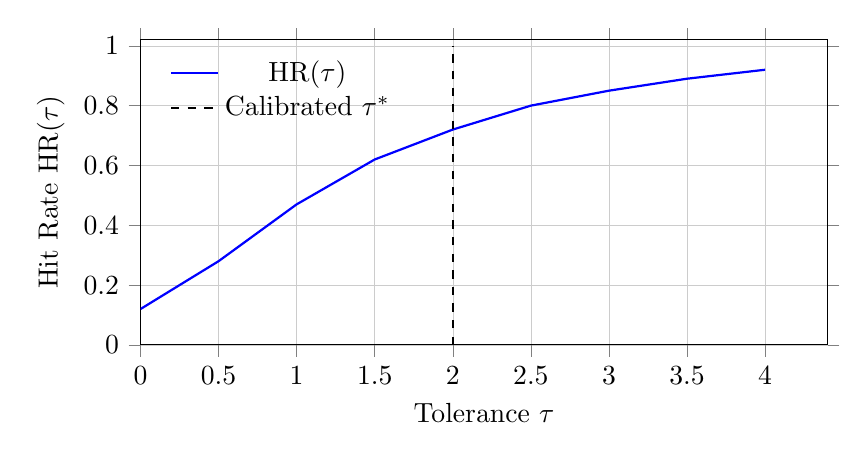
\begin{tikzpicture}
\begin{axis}[
    width=0.85\textwidth,
    height=0.45\textwidth,
    xlabel={Tolerance $\tau$},
    ylabel={Hit Rate $\HR(\tau)$},
    ymin=0, ymax=1.02,
    xmin=0,
    grid=both,
    major grid style={line width=.2pt, draw=gray!40},
    minor grid style={line width=.1pt, draw=gray!20},
    tick align=outside,
    legend style={
        at={(0.03,0.97)},
        anchor=north west,
        draw=none,
        fill=none
    }
]

% --- HR@tau curve (illustrative shape) ---
\addplot[
    thick,
    blue
] coordinates {
    (0.0, 0.12)
    (0.5, 0.28)
    (1.0, 0.47)
    (1.5, 0.62)
    (2.0, 0.72)
    (2.5, 0.80)
    (3.0, 0.85)
    (3.5, 0.89)
    (4.0, 0.92)
};

\addlegendentry{$\HR(\tau)$}

% --- Calibrated tau (example) ---
\addplot[
    dashed,
    thick,
    black
] coordinates {
    (2.0, 0.0)
    (2.0, 1.0)
};

\addlegendentry{Calibrated $\taustar$}

\end{axis}
\end{tikzpicture}

\caption{
Illustrative HR@$\tau$ response surface as a function of tolerance.
The curve shows the monotone increase in hit rate as the acceptable error band
widens, with diminishing marginal gains beyond moderate tolerance levels.
The calibrated tolerance $\taustar$ is selected within a stable region of the
response surface, balancing coverage improvement against tolerance inflation.
}
\label{fig:hrtau_response_surface}
\end{figure}

\subsection{Implications for readiness assessment}
\label{subsec:response_surface_readiness}

Framing \HRtau{} as a response surface clarifies that tolerance-based evaluation
does not yield a single truth but a family of conclusions indexed by $\tauv$.
Readiness judgments based on \HRtau{} therefore depend on where evaluation is
conducted along this surface.

This perspective motivates the use of sensitivity diagnostics and principled
calibration rules.
Rather than fixing $\tauv$ arbitrarily, practitioners can examine how readiness
claims evolve across tolerance values and select reference points that are stable,
interpretable, and aligned with operational standards.

The next section operationalizes this view by introducing grid-based sensitivity
analysis for \HRtau{}, making tolerance dependence explicit and inspectable.
% ----------------------------------------------------------
% SENSITIVITY ANALYSIS
% ----------------------------------------------------------
\section{Grid-Based Sensitivity Analysis}
\label{sec:sensitivity_analysis}

To operationalize the response-surface view of \CWSL{}, we evaluate the metric
across a finite, user-specified grid of candidate cost ratios
$\Rgrid = \{\R_1, \R_2, \ldots, \R_K\}$.
Rather than committing to a single asymmetry assumption, this procedure exposes
how evaluation outcomes vary as $\R{}$ changes, enabling explicit robustness and
stability checks.

This perspective aligns with established principles of sensitivity analysis,
which emphasize understanding how conclusions depend on uncertain assumptions
rather than optimizing parameters in isolation \citep{saltelli2008}.

\subsection{Candidate grid construction}
\label{subsec:grid_construction}

The grid $\Rgrid$ should span the range of cost asymmetries considered plausible
for the application domain.
In practice, $\Rgrid$ is typically chosen as a small set of positive values,
for example $\{0.5, 1.0, 2.0, 3.0\}$ or a denser logarithmic sequence when finer
resolution is required.
The methods discussed here do not rely on any particular spacing or distribution
of grid points; determinism is ensured as long as the grid is fixed.

Importantly, sensitivity analysis does not require that the ``true'' cost ratio
lie exactly on the grid.
The purpose of $\Rgrid$ is not precise estimation, but controlled exploration of
how conclusions change across a range of assumptions.
For this reason, the candidate grid itself should be treated as a governed
artifact, recorded and reported alongside evaluation outputs to ensure
reproducibility and transparency in downstream decision-making.

\subsection{Evaluating the sensitivity curve}
\label{subsec:sensitivity_curve}

For each $\R_k \in \Rgrid$, we compute $\CWSL(\R_k)$ using identical data and
normalization.
The resulting set of pairs
\[
    \{(\R_k, \CWSL(\R_k))\}_{k=1}^{K}
\]
defines a discrete approximation to the continuous response surface discussed in
Section~\ref{sec:response_surface}.

% --- Figure: response surface over the governed grid ---
% ----------------------------------------------------------
% FIGURE: CWSL response surface vs cost ratio R
% ----------------------------------------------------------
\begin{figure}[t]
\centering
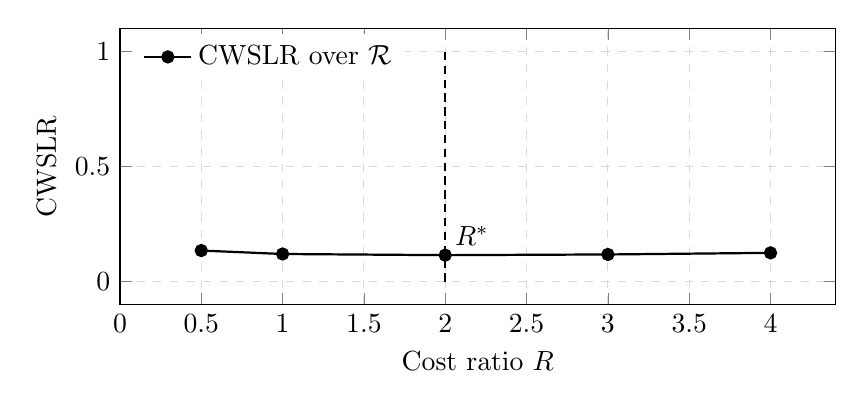
\begin{tikzpicture}
\begin{axis}[
    width=0.88\textwidth,
    height=0.42\textwidth,
    xlabel={Cost ratio $\R{}$},
    ylabel={$\CWSLR{}$},
    xmin=0,
    ymajorgrids=true,
    xmajorgrids=true,
    grid style={dashed,gray!30},
    legend style={draw=none, at={(0.02,0.98)}, anchor=north west},
    legend cell align={left},
]

% --- Placeholder curve (replace with your computed values) ---
% Example grid: R in {0.5, 1.0, 2.0, 3.0, 4.0}
\addplot[
    thick,
    mark=*,
]
coordinates {
    (0.5, 0.135)
    (1.0, 0.120)
    (2.0, 0.115)
    (3.0, 0.118)
    (4.0, 0.125)
};
\addlegendentry{$\CWSLR{}$ over $\Rgrid{}$}

% --- Optional: show calibrated R* as a vertical marker ---
% Replace 2.0 with your calibrated \Rstar{} value.
\addplot[densely dashed, thick] coordinates {(2.0, 0.0) (2.0, 1.0)};
\node[anchor=south west] at (axis cs:2.0, 0.115) {$\Rstar{}$};

% --- Optional: show a "business-chosen" R as a dotted marker ---
% Uncomment and replace 3.0 with your governed default if desired.
% \addplot[dotted, thick] coordinates {(3.0, 0.0) (3.0, 1.0)};
% \node[anchor=south west] at (axis cs:3.0, 0.118) {$\R{}_{\mathrm{gov}}$};

\end{axis}
\end{tikzpicture}
\caption{
Cost-Weighted Service Loss evaluated across a governed candidate grid
$\Rgrid{}$. Marking $\Rstar{}$ on the response surface makes sensitivity and
stability regions explicit and supports auditable model comparison under cost
asymmetry assumptions.
}
\label{fig:cwsl_response_surface}
\end{figure}

Table~\ref{tab:cwsl_sensitivity} reports the corresponding cost decomposition,
making explicit the realized underbuild and overbuild contributions underlying
the response surface and the selection of $\Rstar{}$.

% --- Table: sensitivity + cost decomposition over the governed grid ---
\input{tables/cwsl_cost_ratio_sensitivity_table}

This sensitivity curve provides more information than a single-point estimate.
In particular, it allows practitioners to:
\begin{itemize}[leftmargin=*]
    \item identify regions where \CWSL{} is relatively insensitive to $\R{}$,
    \item detect ranges of $\R{}$ where evaluation outcomes change rapidly,
    \item compare competing forecasts under consistent cost-assumption stress tests.
\end{itemize}

Because the curve is computed from historical residuals alone, it reflects
realized behavior rather than hypothetical model properties.

\subsection{Stability and robustness diagnostics}
\label{subsec:stability_diagnostics}

Sensitivity analysis naturally yields diagnostics that support governed use of
asymmetric metrics.
Flat or gently sloped regions of the sensitivity curve indicate that evaluation
results are robust to moderate mis-specification of $\R{}$.
In contrast, steep segments or sharp changes in curvature signal fragility, where
small differences in assumed cost asymmetry may materially alter conclusions.

These diagnostics are particularly important in model comparison.
If two forecasting approaches cross in ranking at different values of $\R{}$, then
any claim of superiority depends implicitly on a narrow range of cost
assumptions.
Grid-based sensitivity analysis makes such dependencies explicit, allowing
decision-makers to assess whether a chosen model is robust to uncertainty in
operational costs.

\subsection{Role of sensitivity analysis in calibration}
\label{subsec:role_in_calibration}

Sensitivity analysis does not, by itself, prescribe a single ``correct'' cost
ratio.
Instead, it provides the context within which calibration rules can be applied.
By first inspecting the response surface, practitioners can ensure that any
selected $\R{}$ lies in a region that is stable, interpretable, and aligned with
operational priorities.

In the following section, we introduce a deterministic calibration rule that
selects a reference cost ratio by balancing historical underbuild and overbuild
costs across the sensitivity curve, leveraging the structure revealed by the
grid-based analysis.
% ----------------------------------------------------------
% TOLERANCE CALIBRATION RULES
% ----------------------------------------------------------
\section{Tolerance Calibration Rules}
\label{sec:tolerance_calibration}

Framing HR@\(\tau\) as a response surface clarifies that tolerance-based evaluation
does not yield a single, canonical value.
Practical deployment therefore requires a governed rule for selecting a
\emph{reference tolerance} at which readiness is assessed and reported.

This section presents three principled, data-driven tolerance calibration rules.
Each rule operates solely on historical residuals, imposes no model assumptions,
and is deterministic given inputs and a specified tolerance grid.
Importantly, these rules do not estimate a ``true'' tolerance; rather, they define
explicit, auditable conventions for choosing \(\tau\) under different operational
objectives.
This framing follows the broader principle that evaluation criteria should be
treated as first-class decision constructs, rather than tuned parameters
\citep{elkan2001}.

\subsection{Target hit-rate calibration}
\label{subsec:target_hit_rate}

The most direct approach specifies a target hit rate \(\hstar\), representing an
explicit readiness standard.
The reference tolerance is chosen as the corresponding quantile of absolute
forecast errors:
\[
    \taustar = Q\!\left(|e|, \hstar\right).
\]
This rule answers the question:
\emph{What tolerance is required to achieve a desired level of coverage?}

Target hit-rate calibration is highly interpretable and aligns naturally with
service-level definitions.
However, it does not account for the shape of the HR@\(\tau\) response surface and
may select tolerances in regions where readiness conclusions are sensitive to
small changes in \(\tau\).

\subsection{Knee-based calibration}
\label{subsec:knee_calibration}

An alternative approach selects \(\taustar\) at a point of diminishing returns in
the HR@\(\tau\) response surface.
Operationally, this corresponds to a tolerance beyond which additional widening
produces minimal gains in hit rate.

Knee-based calibration emphasizes stability rather than coverage targets.
It is particularly useful when explicit readiness standards are unavailable, or
when robustness to tolerance mis-specification is prioritized over absolute hit
rates.

\subsection{Utility-based calibration}
\label{subsec:utility_calibration}

Utility-based calibration introduces an explicit tradeoff between coverage and
tolerance width.
A simple utility function takes the form
\[
    \Utility(\tauv) = \HR(\tauv) - \lambdau \cdot \left(\frac{\tauv}{\taumax}\right),
\]
where \(\lambdau\) governs the penalty applied to wider tolerances.
The selected tolerance maximizes \(\Utility(\tauv)\) over the candidate grid.

This approach makes preferences explicit and tunable, but requires careful
governance of the penalty parameter to avoid implicit bias toward overly narrow
or overly permissive tolerances.

\subsection{Comparison of calibration rules}
\label{subsec:calibration_comparison}

The three calibration rules are best understood as complementary readiness
primitives rather than competing estimators:

\begin{itemize}[leftmargin=*]
    \item \textbf{Target hit-rate} defines an explicit readiness standard
    (\(\hstar\)) and selects \(\taustar\) to meet that coverage level.

    \item \textbf{Knee detection} selects a stability-oriented reference tolerance
    at diminishing returns on the HR@\(\tau\) response surface.

    \item \textbf{Utility maximization} makes the coverage--tolerance tradeoff
    explicit by introducing a governed penalty \(\lambdau\) on tolerance width.
\end{itemize}

Together, these calibration rules provide a structured vocabulary for tolerance
selection.
They enable readiness assessment to be grounded in explicit assumptions, rather
than implicit defaults, and support consistent reporting and governance across
models, entities, and time periods.

The next section extends tolerance calibration to heterogeneous settings by
allowing entity-level tolerances while introducing safeguards against noise,
instability, and tolerance inflation.
% ----------------------------------------------------------
% ENTITY-LEVEL TOLERANCE AND SAFEGUARDS
% ----------------------------------------------------------
\section{Entity-Level Tolerance and Safeguards}
\label{sec:entity_level}

Operational systems often exhibit heterogeneous error behavior across entities.
Products, locations, services, or demand segments may differ substantially in
their intrinsic volatility, signal-to-noise ratio, or operational tolerance for
forecast deviation.
Applying a single global tolerance $\tauv$ in such settings can obscure
systematic differences and mask localized readiness risks.
This section extends tolerance calibration to the entity level while introducing
explicit safeguards to preserve interpretability and governance.

\subsection{Motivation for entity-specific tolerance}
\label{subsec:entity_motivation}

Let $\entity \in I$ index entities such as items, stores, or service classes.
Historical residuals frequently reveal persistent differences in dispersion
across entities.
Some entities exhibit tight, stable error distributions, while others experience
broader variability due to demand intermittency, substitution effects, or
exogenous shocks.

Allowing entity-specific tolerances $\taui$ enables readiness evaluation to
reflect these differences.
Under a global tolerance, a volatile entity may appear perpetually ``not ready,''
while a stable entity may be evaluated too leniently.
Entity-level calibration therefore improves diagnostic fidelity by aligning
tolerance bands with observed error structure.

However, unconstrained entity-level tolerance selection risks normalizing poor
forecast performance.
Without safeguards, high-variance entities may receive inflated tolerances that
redefine readiness downward rather than improving forecasting behavior.
The objective is thus not maximal flexibility, but controlled heterogeneity.

\subsection{Entity-level calibration rule}
\label{subsec:entity_rule}

For each entity $\entity$, we apply the same calibration rules described in
Section~\ref{sec:calibration} to the subset of residuals associated with that
entity.
Given a minimum sample requirement $\nmin$, we compute
\[
    \taustari
    \in
    \arg\max_{\tauv \in \TauGrid}
    \mathcal{C}_{\entity}(\tauv),
\]
where $\mathcal{C}_{\entity}(\tauv)$ denotes a chosen calibration criterion
(e.g., target hit rate, knee-point, or utility) evaluated using only observations
for entity $\entity$.

Entities with fewer than $\nmin$ valid observations are excluded from
entity-level calibration and assigned no entity-specific tolerance.
This constraint prevents unstable estimates driven by sparse data and makes the
calibration behavior explicit.

\subsection{Global caps and guardrails}
\label{subsec:entity_safeguards}

Even when sufficient data are available, entity-level calibration can yield
excessively large tolerances for entities with persistent forecast dispersion.
To prevent tolerance inflation and preserve cross-entity comparability, we
introduce optional global safeguards.

A common approach is to cap entity-level tolerances by a global reference value
$\taustar$ derived from the full dataset:
\[
    \taustari \leftarrow \min(\taustari, \taustar).
\]
More generally, caps may be defined using high quantiles of the empirical
distribution of entity-level tolerances or through domain-specific maximum
acceptable error thresholds.

Lower bounds may also be imposed to avoid pathological contraction of tolerance
bands in low-variance regimes:
\[
    \taustari \ge \taufloor.
\]
Together, these guards ensure that entity-level calibration refines evaluation
without undermining system-wide readiness standards.

\subsection{Interpretation and reporting}
\label{subsec:entity_interpretation}

Entity-level tolerances should be reported alongside diagnostics including sample
size, achieved hit rate, calibration rule used, and any applied caps or floors.
These diagnostics are essential for distinguishing meaningful heterogeneity from
noise-driven variation.

Importantly, entity-level tolerance calibration is intended primarily as a
\emph{diagnostic and governance tool}, not as a universal deployment default.
In many production environments, a hybrid strategy—global tolerance with
entity-level overrides for well-supported cases—offers the best balance between
fidelity, comparability, and operational discipline.

The next section formalizes governance workflows and diagnostic practices that
support responsible use of tolerance calibration in readiness assessment.
% ----------------------------------------------------------
% GOVERNANCE, DIAGNOSTICS, AND REPORTING
% ----------------------------------------------------------
\section{Governance, Diagnostics, and Reporting}
\label{sec:governance}

Tolerance calibration directly shapes how forecast readiness is defined,
measured, and communicated.
As such, HR@$\tau$ cannot be treated as a purely technical artifact.
This section outlines governance principles and diagnostic practices that ensure
tolerance calibration supports consistent, interpretable, and auditable readiness
assessment.

\subsection{Tolerance as a governed artifact}
\label{subsec:tau_governance}

The tolerance parameter $\tauv$ defines the boundary between acceptable and
unacceptable forecast deviation.
Once calibrated, it establishes a readiness standard that influences model
selection, monitoring, and escalation decisions.
For this reason, $\tauv$ should be treated as a governed artifact rather than an
implicit byproduct of analysis.

At minimum, any deployed tolerance should be accompanied by:
\begin{itemize}[leftmargin=*]
    \item the calibration rule used (e.g., target hit-rate, knee, utility),
    \item the candidate grid $\TauGrid$ over which calibration was performed,
    \item the calibration dataset and sample size,
    \item any applied floors, caps, or exclusions.
\end{itemize}

Recording this information ensures that readiness assessments are reproducible
and that changes in tolerance standards can be traced and reviewed over time.

\subsection{Core diagnostics}
\label{subsec:tau_diagnostics}

Tolerance calibration naturally produces diagnostics that support governance and
interpretation.
Key diagnostics include:
\begin{itemize}[leftmargin=*]
    \item the achieved hit rate $\HRtau(\taustar)$ on the calibration window,
    \item sensitivity of $\HRtau(\tauv)$ around $\taustar$,
    \item the location of $\taustar$ relative to $\taufloor$ and $\taucap$,
    \item the effective sample size used in calibration.
\end{itemize}

These diagnostics allow practitioners to distinguish between robust readiness
standards and fragile thresholds that are sensitive to small changes in error
distribution.
A tolerance that lies in a flat region of the response surface is more defensible
than one chosen near a sharp inflection.

\subsection{Entity-level reporting}
\label{subsec:entity_reporting}

When entity-level tolerances are used, reporting requirements become more
stringent.
Entity-specific tolerances $\taustari$ should always be presented alongside:
\begin{itemize}[leftmargin=*]
    \item the number of observations used for calibration,
    \item the selected calibration rule and parameters,
    \item any global caps or floors applied,
    \item comparison to the global tolerance $\taustar$.
\end{itemize}

Absent this context, entity-level tolerances risk being misinterpreted as
performance endorsements rather than diagnostic signals.
Transparent reporting ensures that heterogeneity is understood as an empirical
property of the system, not an excuse for degraded readiness.

\subsection{Change management and review cadence}
\label{subsec:change_management}

Tolerance calibration should not be updated opportunistically.
Changes to $\tauv$ or $\taustari$ redefine readiness standards and therefore
require explicit review.
A governed process should specify:
\begin{itemize}[leftmargin=*]
    \item the conditions under which recalibration is permitted,
    \item the evaluation windows used for recalibration,
    \item approval or review checkpoints for tolerance changes.
\end{itemize}

In stable environments, tolerances may remain fixed for extended periods.
In rapidly evolving regimes, scheduled recalibration may be appropriate.
In all cases, tolerance drift should be monitored and justified rather than
implicitly accepted.

\subsection{Role in readiness assessment}
\label{subsec:role_in_readiness}

Within the Forecast Readiness Framework, HR@$\tau$ serves as a gatekeeping metric.
It determines whether forecasts satisfy minimum alignment requirements before
more nuanced performance metrics are considered.
Governance of $\tauv$ therefore directly governs what it means for a forecast to
be considered ``ready.''

By pairing tolerance calibration with explicit diagnostics and reporting
standards, organizations can ensure that readiness assessments remain stable,
defensible, and aligned with operational intent.
The next section discusses limitations and non-goals of tolerance-based readiness
metrics, clarifying what HR@$\tau$ is—and is not—designed to capture.
% ----------------------------------------------------------
% ENTITY-LEVEL TOLERANCE AND SAFEGUARDS
% ----------------------------------------------------------
\section{Entity-Level Tolerance and Safeguards}
\label{sec:entity_level}

Operational readiness tolerance is rarely uniform across all entities.
Products, locations, services, or demand segments may differ substantially in
their acceptable deviation from forecast targets.
A single global tolerance $\tauv$ can therefore obscure systematic differences
in readiness behavior and mask localized operational risk.

This section extends tolerance calibration to the entity level while emphasizing
that entity-specific tolerances are primarily a \emph{diagnostic} instrument,
not a default deployment choice.

\subsection{Motivation for entity-specific tolerance}
\label{subsec:entity_motivation}

Let $\entity \in I$ index entities such as items, stores, or service classes.
Historical residual distributions often exhibit persistent differences across
entities.
For example, high-volume or mission-critical entities may require tighter
tolerance bands to maintain readiness, while low-volume or flexible entities
may tolerate wider deviations without operational consequence.

Allowing entity-specific tolerances $\taui$ enables HR@$\tau$ evaluation to
reflect these systematic differences rather than forcing all entities into a
single readiness standard.
However, unconstrained entity-level calibration risks encoding noise rather than
structure, particularly for sparse or volatile entities.

\subsection{Entity-level calibration rules}
\label{subsec:entity_calibration}

For each entity $\entity$, tolerance calibration can be performed using the same
principles introduced at the global level, applied to the entity-specific
absolute error distribution.
Given a candidate grid $\TauGrid$ and sufficient observations, we select
\[
    \taustari \in \TauGrid
\]
according to a governed rule such as target hit-rate, knee detection, or utility
maximization.

Entities with fewer than $\nmin$ valid observations are excluded from
entity-level calibration and assigned no entity-specific tolerance.
This requirement prevents unstable estimates driven by small samples and makes
the scope of calibration explicit.

\subsection{Global caps and guardrails}
\label{subsec:entity_guards}

Even with sufficient data, entity-level calibration can yield excessively large
tolerances when historical errors are highly dispersed.
To prevent tolerance inflation and loss of interpretability, global safeguards
should be applied.

A common strategy is to cap entity-level tolerances relative to a global
reference:
\[
    \taui \leftarrow \min(\taustari, \taucap),
\]
where $\taucap$ may be defined as the globally calibrated tolerance $\taustar$
or a high quantile of the entity-level tolerance distribution.

Additional safeguards may include:
\begin{itemize}[leftmargin=*]
    \item minimum and maximum allowable tolerance bounds,
    \item monotonicity constraints across hierarchical levels,
    \item exclusion of entities with unstable or multimodal error distributions.
\end{itemize}

\subsection{Interpretation and appropriate use}
\label{subsec:entity_interpretation}

Entity-level tolerances should be interpreted as signals of readiness
heterogeneity rather than as prescriptive operational targets.
Large $\taui$ values indicate entities whose historical forecasts frequently
violate tight readiness standards, highlighting candidates for model improvement,
segmentation, or operational review.

Entity-level calibration is therefore best viewed as a diagnostic refinement
layer.
In many deployments, a hybrid approach—global tolerance calibration with
entity-level overrides applied selectively—provides the strongest balance
between fidelity, stability, and governance.

The next section consolidates these ideas by discussing governance practices,
diagnostics, and reporting conventions that support responsible use of tolerance
calibration in production environments.
% ----------------------------------------------------------
% GOVERNANCE, DIAGNOSTICS, AND REPORTING
% ----------------------------------------------------------
\section{Governance, Diagnostics, and Reporting}
\label{sec:governance}

Tolerance calibration plays a foundational role in readiness evaluation.
Because HR@$\tau$ directly defines what constitutes an acceptable deviation
between forecast and realization, the choice of $\tau$ determines the evaluation
context within which readiness is assessed.
As such, tolerance calibration must be governed with the same care as other
operational assumptions, rather than treated as an incidental technical detail.

This section outlines governance principles and diagnostics that support
transparent, stable, and auditable use of HR@$\tau$ in production environments.

\subsection{Separation of calibration and evaluation}
\label{subsec:separation}

A core governance principle is the strict separation between
\emph{calibration} and \emph{evaluation}.
Tolerance calibration determines the reference band $\taustar$ within which
forecast performance is assessed; it does not alter the forecasts themselves
nor adapt the metric to favor a particular model ex post.

Calibration must therefore be performed on a fixed historical window and held
constant when evaluating candidate models or future forecasts.
This separation preserves comparability across models, entities, and time
periods, and prevents circular evaluation in which the tolerance adapts to the
model under inspection.

\subsection{Required diagnostic outputs}
\label{subsec:diagnostics}

Every calibrated tolerance should be accompanied by a minimal set of diagnostic
artifacts.
At a minimum, reporting should include:
\begin{itemize}[leftmargin=*]
    \item the candidate grid $\TauGrid$ used for calibration,
    \item the selected tolerance $\taustar$ (or $\taustari$),
    \item the achieved hit rate $\HR(\taustar)$ on the calibration window,
    \item the number of valid observations used in calibration,
    \item any applied floors, caps, or exclusions.
\end{itemize}

When knee-based or utility-based selection rules are used, additional diagnostics
such as local slope estimates or utility curves should be retained.
These diagnostics ensure that the selected tolerance can be inspected and
justified independently of the calibration procedure itself.

\subsection{Stability and sensitivity checks}
\label{subsec:stability_checks}

Tolerance calibration should not be interpreted as a point estimate.
Instead, practitioners should assess whether the selected $\taustar$ lies in a
region where HR@$\tau$ is locally stable.

Flat regions of the response surface indicate robustness: moderate changes in
$\tau$ do not materially affect readiness conclusions.
Conversely, steep regions signal fragility, where small changes in tolerance
produce large swings in hit rate.
In such cases, broader reporting or more conservative tolerance selection may be
warranted.

These stability considerations are particularly important when tolerances are
used as contractual thresholds, service-level objectives, or escalation triggers.

\subsection{Entity-level reporting and safeguards}
\label{subsec:entity_reporting}

When entity-level tolerances are computed, governance requirements become more
stringent.
Entity-level outputs should always be reported alongside:
\begin{itemize}[leftmargin=*]
    \item entity-specific sample sizes,
    \item achieved hit rates at $\taustari$,
    \item any global caps or overrides applied,
    \item the corresponding global reference tolerance $\taustar$.
\end{itemize}

This contextual information is essential for distinguishing meaningful readiness
heterogeneity from noise-driven variation.
Absent such diagnostics, entity-level tolerances risk being misinterpreted as
prescriptive targets rather than descriptive indicators.

\subsection{Auditability and lifecycle management}
\label{subsec:auditability}

Tolerance calibration should be treated as a governed artifact with a defined
lifecycle.
Calibration inputs, rules, and outputs should be versioned, timestamped, and
recomputed only when material changes occur in demand behavior, forecast systems,
or operational objectives.

In regulated or high-stakes environments, the ability to reconstruct the
calibration decision—given the historical data and declared rules—is essential.
HR@$\tau$ calibration is therefore designed to be fully deterministic and
reproducible, supporting retrospective audit and forward-looking governance.

Taken together, these practices ensure that tolerance calibration strengthens
readiness assessment rather than obscuring it.
In the next section, we situate HR@$\tau$ calibration within the broader
Forecast Readiness Framework and clarify its role alongside other readiness
primitives.
% ----------------------------------------------------------
% LIMITATIONS AND NON-GOALS
% ----------------------------------------------------------
\section{Limitations and Non-Goals}
\label{sec:limitations}

The tolerance calibration methods presented in this note are designed to support
transparent, governed readiness evaluation.
They are intentionally constrained in scope.
This section clarifies what HR@$\tau$ calibration does \emph{not} attempt to do
and outlines limitations that should be considered when deploying these methods
in practice.

\subsection{Not a forecasting objective}
\label{subsec:not_objective}

HR@$\tau$ and its calibration rules are evaluation constructs, not training
objectives.
They are not intended to replace loss functions used during model estimation,
nor to serve as direct optimization targets.
In particular, calibrating $\tau$ does not imply that forecasts should be
trained to maximize hit rate within a tolerance band.

Using HR@$\tau$ calibration as a training objective risks collapsing readiness
evaluation into a form of implicit over-smoothing, where forecasts are biased
toward tolerance compliance rather than operational alignment.
The methods in this note assume that forecasting models are trained independently
and evaluated within a fixed, governed tolerance context.

\subsection{Dependence on historical behavior}
\label{subsec:historical_dependence}

All calibration rules described here rely exclusively on historical forecast
errors.
As a result, calibrated tolerances reflect past system behavior and error
distributions.
When demand regimes, forecasting methods, or operational constraints change
materially, previously calibrated tolerances may become stale.

This limitation is not unique to HR@$\tau$, but it underscores the importance of
treating tolerance calibration as a periodic, versioned process rather than a
one-time decision.
Recalibration should be triggered by substantive changes in forecast dynamics,
not by short-term performance fluctuations.

\subsection{Sensitivity to grid specification}
\label{subsec:grid_sensitivity}

Grid-based calibration inherits sensitivity to the choice of candidate tolerance
set $\TauGrid$.
While the methods are deterministic for a fixed grid, different grids can yield
different calibrated tolerances, particularly in regions where the response
surface is steep.

For this reason, the grid itself must be governed and reported alongside results.
The methods presented here do not attempt to infer a continuous optimum or to
adaptively refine the grid; such extensions may be appropriate in some settings
but would introduce additional complexity and assumptions beyond the scope of
this note.

\subsection{Interpretation under sparse data}
\label{subsec:sparse_data}

Entity-level tolerance calibration is especially sensitive to sample size.
When the number of observations per entity is small, calibrated tolerances may
reflect noise rather than structural readiness differences.
Minimum sample thresholds and global caps mitigate this risk but do not eliminate
it entirely.

Consequently, entity-level HR@$\tau$ calibration should be interpreted primarily
as a diagnostic signal.
Its outputs should inform investigation and segmentation decisions rather than be
applied mechanically or universally.

\subsection{What HR@$\tau$ does not capture}
\label{subsec:not_capture}

HR@$\tau$ captures whether forecast errors fall within an acceptable band, but it
does not encode the magnitude of errors outside that band.
Two forecasts with identical hit rates may differ substantially in the severity
of their misses.

For this reason, HR@$\tau$ is not a substitute for magnitude-sensitive metrics
such as CWSL, NSL, or UD.
Within the Forecast Readiness Framework, tolerance-based metrics must be
interpreted alongside cost-weighted and depth-sensitive measures to form a
complete readiness assessment.

Taken together, these limitations reinforce the intended role of HR@$\tau$:
a governed, interpretable readiness primitive that defines tolerance boundaries,
not a standalone measure of forecast quality or a replacement for operational
loss modeling.
% ----------------------------------------------------------
% RELATIONSHIP TO FORECAST READINESS
% ----------------------------------------------------------
\section{Relationship to Forecast Readiness}
\label{sec:relationship_to_readiness}

Within the Forecast Readiness Framework (FRF), readiness is defined by the degree
to which forecasts align with operational tolerance, risk posture, and decision
consequences.
Accuracy alone is insufficient: readiness depends on whether forecast errors
fall within acceptable bounds and whether deviations beyond those bounds are
manageable.

HR@$\tau$ formalizes this notion by introducing an explicit tolerance parameter
$\tau$ that defines what constitutes an acceptable forecast deviation.
For a fixed tolerance, HR@$\tau$ measures the fraction of forecasts whose errors
lie within operational limits.
However, without principled calibration of $\tau$, readiness assessment becomes
ambiguous and potentially inconsistent across entities, horizons, or evaluation
cycles.

Tolerance calibration addresses this gap by transforming HR@$\tau$ from a
descriptive statistic into a governed readiness construct.
By selecting $\tau$ using transparent, data-driven rules, the evaluation
environment itself becomes explicit and auditable.
This separation between calibration and evaluation preserves interpretability
and prevents post hoc adjustment of tolerance to favor particular models or
outcomes.

From a readiness perspective, calibrated tolerance defines the \emph{acceptance
envelope} within which forecast performance is judged.
Together with cost-ratio calibration for \CWSL{}, tolerance calibration determines
the evaluation space over which readiness is assessed.
These calibration steps operate upstream of metric computation and ensure that
subsequent scores reflect consistent operational assumptions.

Entity-level tolerance calibration further exposes structural heterogeneity in
readiness.
Entities with narrow calibrated tolerances exhibit low error tolerance and
require precise forecasting to maintain readiness, while entities with broader
tolerances may absorb larger deviations without material impact.
Importantly, these differences are diagnostic signals rather than prescriptions;
they inform segmentation, investigation, and governance decisions rather than
mandating entity-specific deployment behavior.

Within FRF, HR@$\tau$ calibration operates alongside other readiness primitives
such as cost-weighted loss (\CWSL{}), shortfall avoidance (NSL), and loss depth
(UD).
Each primitive captures a distinct aspect of operational risk.
Tolerance calibration specifies \emph{whether} errors are acceptable, while
cost-weighted metrics quantify \emph{how costly} unacceptable errors are when
they occur.

In this sense, HR@$\tau$ calibration is not a tuning convenience but a readiness
primitive.
It defines the tolerance boundary against which forecasts are evaluated,
supporting consistent, explainable, and decision-aligned readiness assessment
across models, entities, and time horizons.
% ----------------------------------------------------------
% CONCLUSION
% ----------------------------------------------------------
\section{Conclusion}
\label{sec:conclusion}

HR@$\tau$ provides a direct and interpretable measure of forecast readiness by
explicitly encoding tolerance for error.
However, without principled selection of the tolerance parameter, readiness
assessment risks becoming arbitrary, unstable, or vulnerable to post hoc
adjustment.
This technical note reframes tolerance selection as a governed calibration
problem rather than a modeling choice.

By treating HR@$\tau$ as a response surface over tolerance, we introduce a
systematic framework for sensitivity analysis and deterministic calibration.
Quantile-based targets, knee detection, and utility-based rules provide
complementary mechanisms for selecting $\tau$ based on observed forecast
behavior, operational preferences, and governance constraints.
Entity-level extensions and safeguards further support responsible application
in heterogeneous settings.

Together with cost-ratio calibration for \CWSL{}, tolerance calibration defines
the evaluation envelope within which readiness is assessed.
These calibration primitives operate upstream of metric computation and ensure
that readiness metrics are applied within a consistent, auditable, and
operationally meaningful context.

The result is a readiness evaluation framework that separates measurement from
assumption, supports transparent governance, and aligns forecast assessment with
real operational tolerance.
As part of the broader Forecast Readiness Framework, calibrated HR@$\tau$ enables
forecast evaluation that is not only accurate, but decision-aligned and fit for
deployment.

% ----------------------------------------------------------
% REFERENCES
% ----------------------------------------------------------
\bibliographystyle{plainnat}
\bibliography{references}

\end{document}